\documentclass{article}
\usepackage{graphicx}
\usepackage{hyperref}
\usepackage{float}
\usepackage{url}
\usepackage{cite}
\usepackage[utf8]{inputenc}
\usepackage[a4paper, margin=2cm]{geometry}

\title{Relatório sobre o Protocolo HTTP}
\author{Nicolas Chagas Souza}
\date{\today}

\begin{document}

\maketitle

\section{Introdução}

\section{Protocolo HTTP}

O protocolo HTTP encontra-se na camada de aplicação dos modelos TCP/IP e OSI.

\begin{figure}[H]
    \centering
    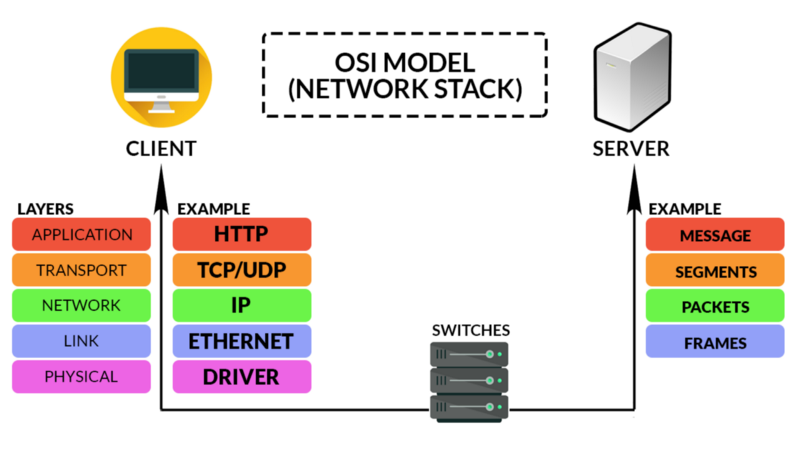
\includegraphics[width=\textwidth]{./assets/osi.png}
    \caption{Modelo OSI. (Fonte: freeCodeCamp \cite{freecodecamp})}
\end{figure}

\subsection{Arquitetura Cliente-Servidor}

\subsubsection{Cliente}

\begin{itemize}
    \item Dispositivo ou aplicativo que solicita serviços ou recursos.
    \item Geralmente um navegador web, mas pode ser qualquer aplicativo que faça
          requisições a servidores.
\end{itemize}

\subsubsection{Servidor}

\begin{itemize}
    \item Dispositivo ou programa que fornece serviços ou recursos em resposta às
          solicitações do cliente.
    \item Pode hospedar sites, aplicativos, ou dados.
\end{itemize}

\subsubsection{Comunicação}

\begin{figure}[H]
    \centering
    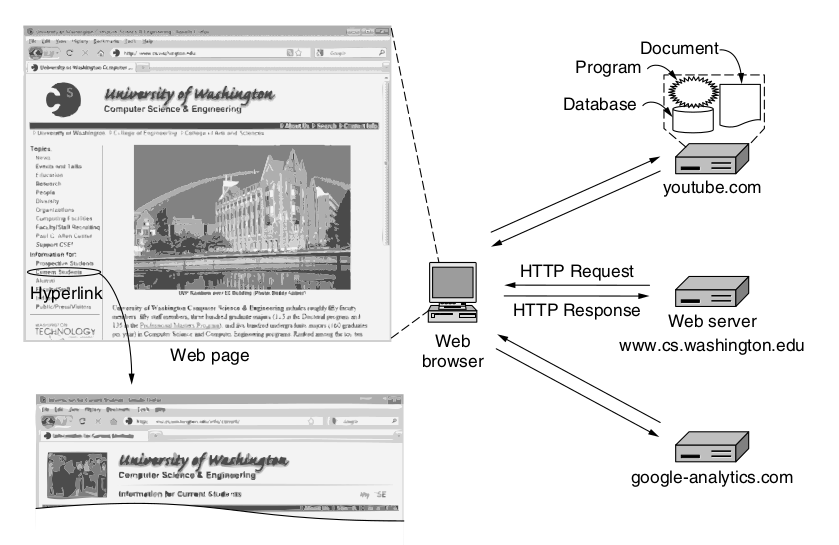
\includegraphics[width=\textwidth]{./assets/3510.png}
    \caption{Arquitetura da web. (Fonte: Tanenbaum \cite{tanenbaum})}
\end{figure}

\paragraph{Requisição (Request)}

\begin{itemize}
    \item O cliente envia uma requisição ao servidor para obter informações ou realizar
          uma ação.
    \item Utiliza o protocolo HTTP para estruturar e enviar a requisição.
\end{itemize}

\paragraph{Resposta (Response)}

\begin{itemize}
    \item O servidor processa a requisição e envia uma resposta de volta ao cliente.
    \item A resposta contém os dados solicitados ou informações sobre a execução da ação.
\end{itemize}

\begin{figure}[H]
    \centering
    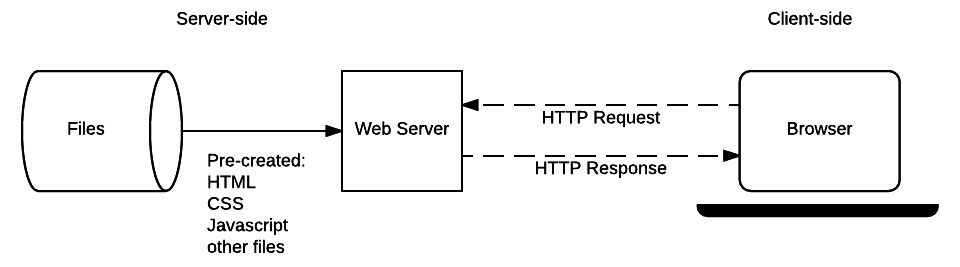
\includegraphics[width=\textwidth]{./assets/5859.png}
    \caption{Arquitetura Cliente-Servidor. (Fonte: MDN \cite{mdn-client-server})}
\end{figure}

\section{O Protocolo HTTP}

\begin{itemize}
    \item Desenvolvido por Tim Berners-Lee entre 1989 e 1991, no CERN (Organização
          Europeia para a Pesquisa Nuclear), o HTTP é o protocolo subjacente à World Wide
          Web.
    \item Concluído até o final de 1990, marcando o início oficial da World Wide Web em
          agosto de 1991.
    \item Define as regras para a comunicação entre cliente e servidor na web.
    \item Permite a transferência de documentos hipertexto, como páginas web.
\end{itemize}

\begin{figure}[H]
    \centering
    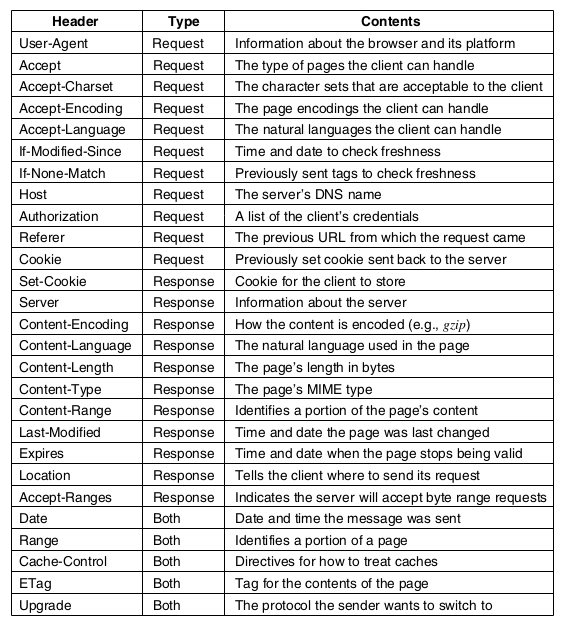
\includegraphics[width=\textwidth]{./assets/1312.png}
    \caption{Alguns cabeçalhos HTTP. (Fonte: Tanenbaum \cite{tanenbaum})}
\end{figure}

\begin{itemize}
    \item Requisições e respostas HTTP têm um formato específico com cabeçalhos e,
          opcionalmente, um corpo com dados.
\end{itemize}

\begin{figure}[H]
    \centering
    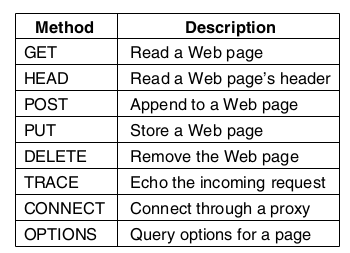
\includegraphics[width=\textwidth]{./assets/1035.png}
    \caption{Métodos HTTP. (Fonte: Tanenbaum \cite{tanenbaum})}
\end{figure}

\begin{itemize}
    \item Cada requisição é independente das anteriores, sem armazenamento de estado
          entre transações (\textit{stateless}).
    \item Define diferentes métodos, como \texttt{GET} para obter dados, \texttt{POST}
          para enviar dados ao servidor, etc.
\end{itemize}

\begin{figure}[H]
    \centering
    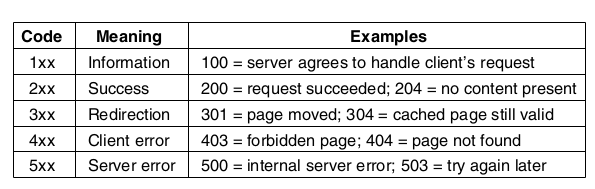
\includegraphics[width=\textwidth]{./assets/1141.png}
    \caption{Códigos de status. (Fonte: Tanenbaum \cite{tanenbaum})}
\end{figure}

\begin{itemize}
    \item A versão do HTTP, o código de status e a frase de motivo acompanham as
          respostas na linha de status.
    \item Códigos de status (números de 3 dígitos) acompanhados de frases de motivo
          resumem o significado do código.
\end{itemize}

\section{Versões do Protocolo HTTP}

\begin{itemize}
    \item Clientes e servidores podem usar versões diferentes, e a versão é indicada na
          primeira linha de requisições e respostas.
\end{itemize}

\section{Experimento}

\subsection{HTTP 1.0}
\subsection{HTTP 1.1}
\subsection{HTTP 2.0}

\section{Conclusões}
\subsection{Opiniões dos Participantes}
Nesta seção, cada participante pode expressar suas opiniões sobre o
experimento, destacando as dificuldades encontradas, limitações percebidas e
fornecendo uma autoavaliação.

\subsection{Diferenças entre as Versões}
Destacamos as principais diferenças entre as versões do protocolo HTTP
discutidas neste relatório.

\subsection{Considerações Finais}
Resumimos as conclusões gerais do experimento.

% \section{Referências}
% \begin{itemize}

%     https://developer.mozilla.org/en-US/docs/Web/HTTP/Basics_of_HTTP/Evolution_of_HTTP
%     https://www.baeldung.com/cs/http-versions
%     https://www.w3.org/Protocols/History.html
%     https://www.ibm.com/docs/en/cics-ts/5.3?topic=concepts-http-protocol
%     http://www.tcpipguide.com/free/t_HTTPOverviewHistoryVersionsandStandards.htm

%     \item Autor1, Nome1. \textit{Título do Livro}. Editora, Ano.
%     \item Autor2, Nome2. \textit{Título do Artigo}. Nome da Revista, Ano.
%     \item Site1: \href{http://www.exemplo.com}{Exemplo}
% \end{itemize}

\bibliographystyle{plain}
\bibliography{refs}

\end{document}
